
\section{State of the Art}
\label{sec:state}

\subsection{Big data}

As I have pointed out in section \ref{sec:problem}, this platform has to handle
a huge amount of raw data. This concept is known as {\bf Big data}. There is
no specific definition of Big data. However, we can see Big data as a term that
applies to any collection of data sets so large and complex that it becomes
difficult to manipulate this data with traditional approaches.

This term is relatively new, and it brings with it a set of challenges that
are not trivially solvable. This concept has been applied to a wide variaty of
fields. Some examples:

\mylist
  \item {\bf Science}: the Large Hadron
Collider\footnote{http://en.wikipedia.org/wiki/Large\_Hadron\_Collider} has a
set of 150 sensors that deliver data 40 times per second each. After applying
some filters, we have around 100 collisions of interest per second. This means
that the LHC has to handle 500 exabytes of data every day.
  \item {\bf Government}: it is known that the Obama administration has used
supercomputers and Big data techniques to address important problems faced by
the government.
  \item {\bf Private sector}: companies such as Google, Facebook, Twitter,
Amazon, etc. use big data technologies to handle the large quantity of data
that their servers receive.
\mylistend

This idea of Big data has revolutionized technology since it is a very
important topic and that it has to be fixed. To fix this, we can basically do
two things:

\begin{enumerate}
  \itemsep0em
  \item Add more {\bf hardware}. This is the simplest solution: if one server
cannot handle the flow of data, let us add more servers. The problem of this is
that it might not always work and that it will make the infrastructure more
expensive to maintain.
  \item Improve the {\bf algorithms} behind the handling of data flows. This is
what an engineer should always do before blindly adding new servers. Algorithms
will usually apply to how the tasks are distributed across the infrastructure
and how this data is then treated.
\end{enumerate}

In this chapter I will be focusing the second solution, since it is the most
interesting from an engineering stand point.

\subsection{MapReduce}

The first algorithm to tackle the Big data problem was the {\bf MapReduce}
algorithm. This algorithm was introduced by Google in the paper ``MapReduce:
Simplified Data Processing on Large Clusters''.

This is a two-steps, parallel, distributed algorithm that works on {\it
clusters} and {\it grids}. The data can be stored either in a filesystem or in a
database. The two steps are as follows:

\begin{enumerate}
  \itemsep0em
  \item {\bf Map}: The master node takes the input, divides it into smaller
problems and distributes them to worker nodes. A worker node may do this again
in turn.
  \item {\bf Reduce}: The master node collects all the answers to all the
sub-problems and combines them in some way to form the output.
\end{enumerate}

This algorithm can be visualized as follows:

\begin{center}
  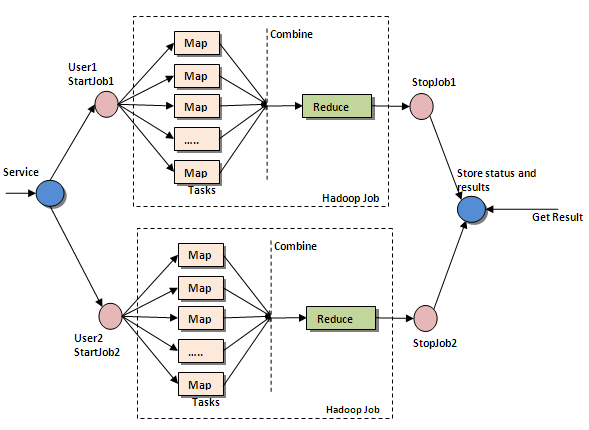
\includegraphics[scale=0.8]{overview/images/mapreduce.png}
\end{center}

In the example above, two users start a Hadoop job. As we can see, a job
consists of the map and reduce steps.

Many programs and frameworks that implement the MapReduce algorithm have
appeared since the initial announcement from Google. For example, some
well known programs implementing in some way or another the MapReduce algorithm
are: Hadoop, Cassandra and MongoDB.

\subsection{Storm}
\label{sec:state_storm}

Hadoop\footnote{http://hadoop.apache.org/} is the most notable implementation of
the classic MapReduce algorithm. It guarantees reliability and scalability.
Moreover, Hadoop is really fast and efficient, and because its popularity some
big projectes like Apache Hive or Apache Spark are closely related to it.

However, Hadoop has one major drawback: it uses {\bf batch processing}. This is
not a flaw or a weakness, it is like this by design. Hadoop is designed to
process data through batches: handling large amount of data in a single round.
But sometimes the data to be processed is not available yet. This happens when
you receive a lot of data that has to be processed in realtime: you do not have
the data available right now, but you do not want to setup a batch for all the
packets of data to come.

Some people have tried to hack Hadoop to workaround these issues. However, all
the attempts have failed so far because:

\mylist
  \item It is {\bf tedious}. People have to implement message queues and
protocols around them.
  \item There is no real {\bf fault tolerance}. Complex systems have to be
developed in order to handle fault tolerance gracefully. All the attempts on
this have failed horribly.
  \item It does not {\bf scale}. When you add or remove more servers, you have
to manually do the changes. This happens quite frequently, so it is a pain that
the developer has to usually face.
\mylistend

As we have seen, there is no hack that will turn Hadoop into a
realtime system; realtime data processing has a fundamentally different set of
requirements than batch processing. Therefore we need some sort of ``Hadoop of
realtime''. Two projects aspired to get this ``title'':

\begin{enumerate}
  \itemsep0em
  \item Yahoo! {\bf S4}. One of the first implementations of this idea. It is
now under the umbrella of the Apache foundation. However, as of the writing of
this document, this project seems to have died: the development has stopped
since a couple of years ago, lack of documentation, etc.
  \item Twitter {\bf Storm}. It is the natural competitor of S4, and the one
that is still alive and in production in companies such as Twitter. It is now
under the umbrella of the Apache foundation just like S4.
\end{enumerate}

I picked Storm for this project since there is no real alternative to it and
quite honestly Storm is really good at it. Storm has the following main points:

\mylist
  \item It {\bf scales}. Companies such as Twitter or Zookeeper have Storm in
production and they get nice results. As an example, an initial Storm
application on a cluster of 10 nodes can handle 1,000,000 messages per second.
  \item It guarantees {\bf no data loss}.
  \item It is {\bf fault-tolerant}. If some task fails, it will be re-assigned
later on the execution of the application.
\mylistend

Each Storm application has to define a {\bf topology}. This is accomplished
with the idea of {\bf spouts} and {\bf bolts}. Spouts and bolts are the way to
specify how data streams have to be consumed. Spouts are used to fetch the data
that has to be processed and bolts consume this data in order to get results.
There can be several spouts and bolts in a topology. Bolts get the data from
spouts or from other bolts. The following picture shows how Storm understands
the notion of topology:

\begin{center}
  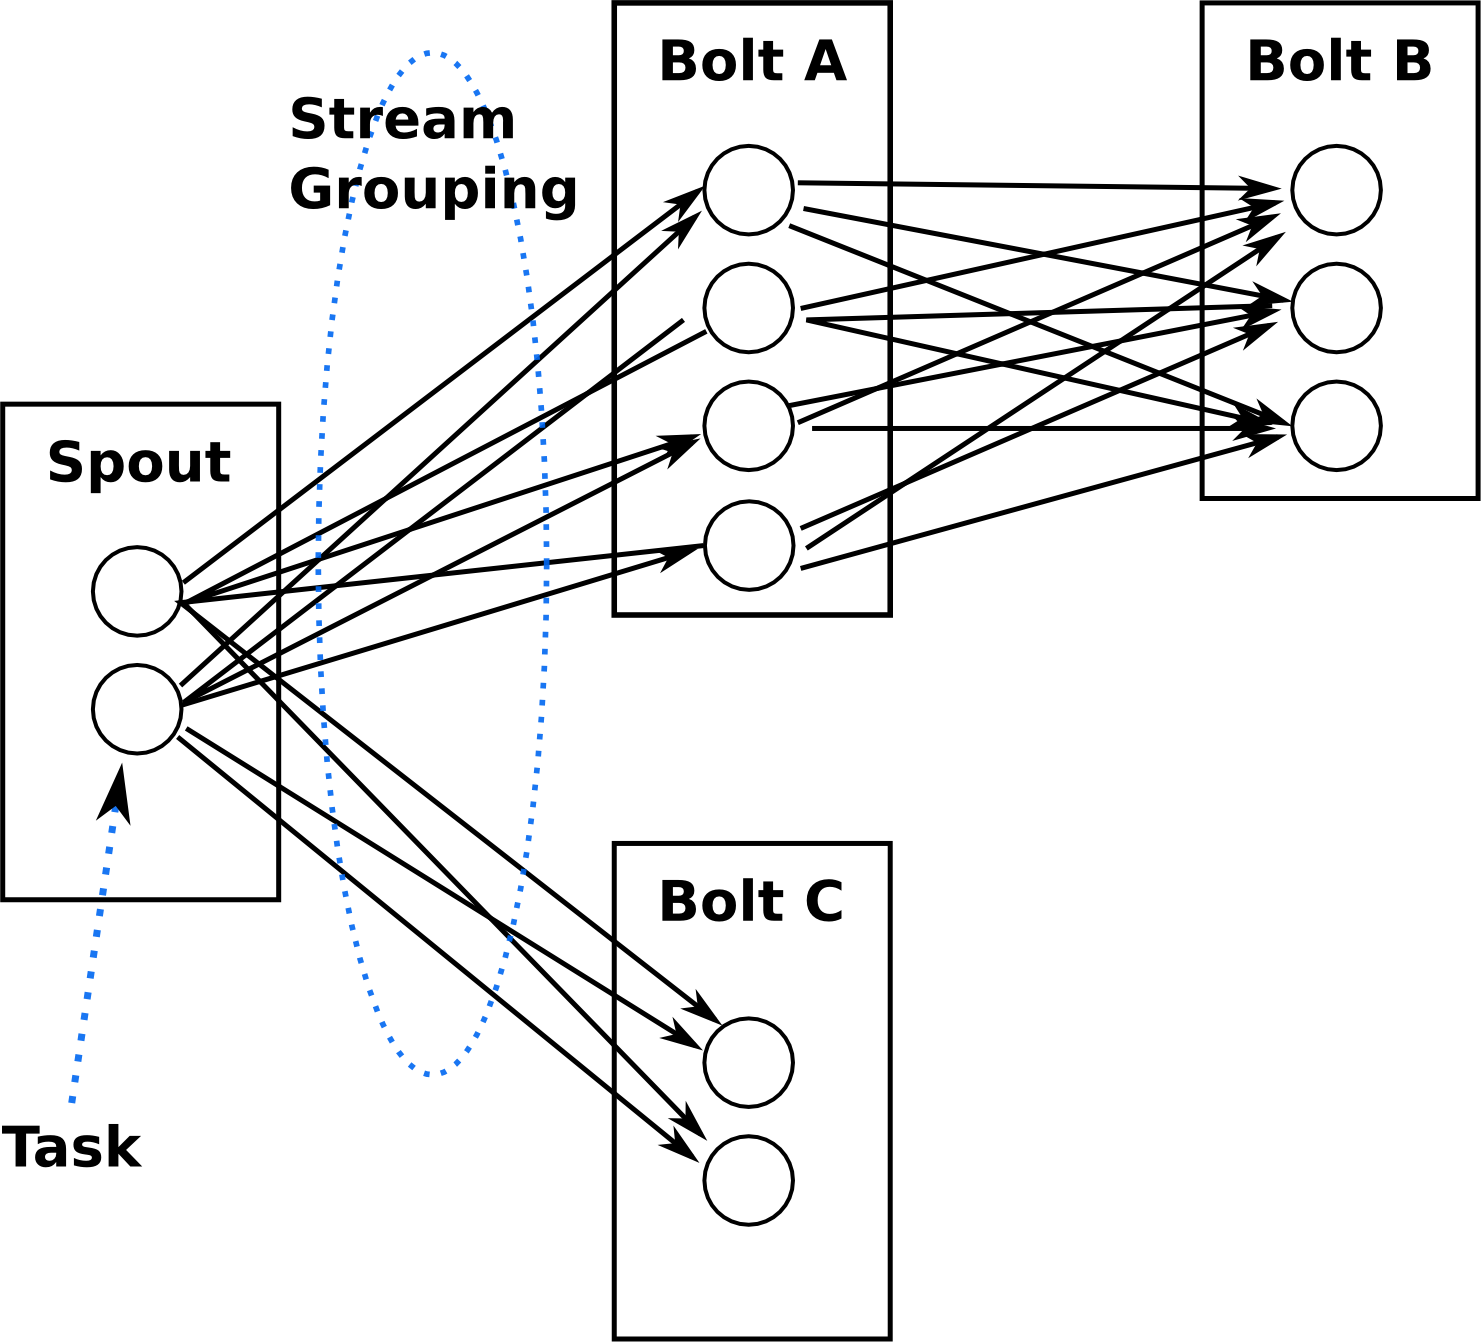
\includegraphics[scale=0.25]{overview/images/storm.png}
\end{center}
